\chapter{Lösung}
Dieses Kapitel befasst sich mit den Möglichkeiten und Lösungsansätze, zu den Problemstellungen aus Kapitel \ref{ch:problem}. Anhand von Beispielen wird verdeutlicht, wie gewisse Anforderungen umgesetzt werden könnten und wurden.

\section{Meta-Model}
Nach der Anforderungsanalyse, wurden alle relevanten Informationen erkannt und zusammen gestellt. Diese Zusammenstellung an Daten, welche die Applikation beschreiben wird Meta-Model genannt.

\subsection{Kompatibilität mit \acs{gemara} und andern möglichen Clients}

Um die Kompatibilität mit \acf{gemara} zu waren, wurde das Enfield-Meta-Model untersucht. Mit Hilfe dieser Untersuchung konnte festgestellt werden, an welcher Stelle zusätzliche Informationen für die Clients am sinnvollsten eingebaut werden können. So das diese den Ablauf der Applikation gut beschreiben und an den benötigten Stellen alle relevanten Informationen für den Software-Generator zur Verfügung stellt.

Die Abbildung \ref{fig:enfield-model} zeigt die vereinfachte Model-Klasse des Enfield-Meta-Models. 
In dieser Klasse sind bereits die wichtigsten Informationen wie zum Beispiel der Name der Applikation, oder unter welchem Package diese zu finden ist. Neben diesen grundsätzlichen Informationen liefert die Model-Klasse auch den Startpunkt des endlichen Automaten, welcher die Anwendung beschreibt. Dieser Startpunkt ist der \textit{GetDispatcherState}. Dieses Objekt besitzt das Attribut \textit{transitions}. Dieses Attribut beschreibt, welche States auf den Dispatcher-State folgen können. Jeder dieser folgenden States, besitzt wiederum eine Collection mit Transitionen, die auf die nachfolgenden States verweisen. So wird mit Hilfe der Transitionen und der States der endliche Automat der Anwendung beschrieben. Der Generator kann diese Beschreibung nutzen, um zu entscheiden in welcher Reihenfolge, welche Klassen generiert werden müssen.

\begin{figure}[H]
	\begin{center}
		\includegraphics[width=0.86\textwidth]{images/Enfield-Meta-Model.png}
		\caption{Vereinfachter Aufbau des Enfield-Meta-Models}
		\label{fig:enfield-model}
	\end{center}
\end{figure}

Um jetzt zusätzlich benötigten Informationen für die Android Applikation in dieses bestehende Modell einzubauen, gibt es zwei Möglichkeiten.

\subsection{Eigenes Android-Meta-Model}

Es besteht die Möglichkeit die Model-Klasse um ein Attribut \textit{Android-Meta-Model} zu erweitern.
Die Abbildung \ref{fig:android-model} stellt zeigt schemenhaft ein Beispiel wie ein Android-Meta-Model aussehen könnte. Auffällig hierbei ist das viele Informationen, die das Enfield-Model bereits liefern würde, hier noch einmal explizit beschrieben werden muss. Ein Beispiel wären die Transitionen, zwischen den Fragmenten beziehungsweise zwischen den Activities. 


\begin{figure}[H]
	\begin{center}
		\includegraphics[width=0.86\textwidth]{images/Android-Meta-Model.png}
		\caption{Möglicher Aufbau eines Android-Meta-Models}
		\label{fig:android-model}
	\end{center}
\end{figure}

Der Nutzer des Software-Generators, muss also ziemlich viel über den Ablauf und die Funktionsweiße einer Android-Anwendung wissen, um diesen Generator sinnvoll verwenden zu können.
Dabei bleibt zusätzlich noch die Möglichkeit, das der Nutzer eigens geschriebene Metohden in das Model einpflegen kann. John Abou-Jaoudeh at al., haben in ihrer Arbeit \textit{A High-Level Modeling Language for Efficent Design, Implementation, and Testing of Android Applications} ein Meta-Model entwickelt, welches genau solche Features unterstützt \cite{abou2015high}.

Der Vorteil einer solchen Erweiterung des Enfield-Models ist, das alle benötigten Daten für die Android Anwendung an einer Stelle zu finden sind. Auch hat der Nutzer die Möglichkeit an manchen Stellen eigene Methoden einzufügen und somit ist er in der Lage das Verhalten der App weiter zu individualisieren.

Jedoch überwiegen in diesem Fall die Nachteile. Ein Nachteil dieses Vorgehens ist, die redundante Beschreibung des Programm-Ablaufes. Einmal im Android-Meta-Model und einmal im Enfield-Meta-Model. Bei jeder Änderung gilt dies zu berücksichtigen. 
Der nächste Nachteil ist der Nutzer des muss sich in der Entwicklung von Android Anwendungen auskennen. Er muss genau das Zusammenspiel von ViewHoldern, Adaptern, Fragments und Activities kennen. Er muss wissen wie diese ineinandergreifen und wann welche Aktionen ausgelöst werden müssen. Weiterhin sollte er ein Grundsätzliches Verständnis für das \acf{mvc} Pattern besitzen, welches bei der Entwicklung von Android Applikationen anwendung findet.
Ein weiterer Nachteil ist die Beschränkung des Models auf Android. Wird das Enfield-Model um ein Android-Meta-Model erweitert, so muss dieses für jeden einzelnen Client geschehen. Soll der Generator beispielsweise um Polymer-Webkomponente oder einer iOS-Anwendung erweitert werden, so müsste für jede einzelne Art von Client, das Enfield-Model mit einem Entsprechenden Meta-Model erweitert werden.

\subsection{Allgemeine Erweiterungen des Enfield-Models an entsprechender Stelle}

In dieser Arbeit wurde sich für die Variante entschieden, das Enfield-Model an ihren \textit{SingleResourceViews} zu erweitern.
Wird diese Klasse um die  Attribute, die benötigt werden Attribute erweitert, so erhält der Generator die benötigten Ressourcen immer zur rechten Zeit.

Wird beispielsweise eine Instanz eines \textit{GetPrimarySingleResourceByIdStates} erzeugt, und dessen \textit{SingleResourceView} enthält alle notwendigen Informationen, um die View in der Android Anwendung zu beschreiben. Kann der Generator mit Hilfe der Transitionen über die States iterieren und verfügt an jedem State über alle benötigten Informationen, um den aktuellen State in der Anwendung generieren zu lassen.

Bei dieser Methode befinden sich alle State-spezifischen Daten direkt am State. Jedoch gibt es neben diesen spezifischen Daten auch Daten, welche die komplette Applikation betreffen, muss das Enfield-Model noch an einer andern Stelle erweitert werden. 
Hierfür erscheint es sinnvoll die Erweiterung direkt in der Model-Klasse vorzunehmen. So kann der Generator schon am Anfang auf diese Daten zugreifen und diese verarbeiten.

Die Abbildung \ref{fig:enfield-model-extended} zeigt das Enfield-Model, welches um die oben genannten Informationen erweitert wurden.

\begin{figure}[H]
	\begin{center}
		\includegraphics[width=0.86\textwidth]{images/Enfield-Meta-Model-Erweitert.png}
		\caption{Vereinfachter Aufbau des erweiterten Enfield-Meta-Models}
		\label{fig:enfield-model-extended}
	\end{center}
\end{figure}

Der Nachteil dieser Methode ist, das die Informationen an mehr als einer Stelle im Enfield-Modell zu finden sind. Sollten die Informationen zu den Clients verändert werden, so sind Änderungen an der SingleResourceView-Klasse und in der Model-Klasse nötig. Die Vorteile wurden jedoch oben schon einmal erwähnt. Der Generator kann das Model als Fahrplan nutzen und weiß genau wann er welche Klassen für die Android Anwendung erzeugen muss. Er kann auch mit Hilfe der Transitionen bestimmen wie der Verlauf innerhalb der Anwendung ablaufen soll.

\newpage
\subsection{Analyse der benötigten Dateien für das Meta-Model}

Nachdem identifiziert wurde, an welchen Stellen das Enfield-Model erweitert werden soll, muss noch analysiert werden, welche Informationen an diesen Stellen zur Verfügung stehen müssen. Bei dieser Analyse muss auch ein Augenmerk darauf gelegt werden, wie man die Informationen so aufbereitet, dass diese nicht nur eine Android-Applikation, sondern mögliche andere Clients unterstützen.

Die Analyse in dieser Arbeit beschränken sich auf die Clients Android und Polymere-Webkomponente. Bei beiden wird das \acf{ui} nach den Guidelines,des von Google entwickelten Material Design, erstellt \cite{material}. Diese Guidelines schreiben bereits viele nötigen Informationen für die Oberflächengestaltung vor. So wird beispielsweise definiert, das Einträge in einer Liste, als Karte dargestellt werden sollen. Abstände und Icons werden ebenfalls festgelegt.

\subsubsection{CardView}

\begin{figure}[H]
	\begin{center}
		
\includegraphics[width=0.86\textwidth]{images/card.png}
		\caption{Beispiel einer CardView aus einer Liste von Dozenten nach Material Design Guidelines.}
		\label{fig:card}
	\end{center}
\end{figure}

\newpage

\begin{lstlisting}[label=lst:braun_json,
language=json,
firstnumber=1,
caption=Demo Daten eines Dozenten.]	
...			   
{
	"address": "Sanderheinrichsleitenweg 20 97074 Wuerzburg",
	"chargeUrl": {
		"href": "https://apistaging.fiw.fhws.de/mig/api/lecturers/4/charges",
		"rel": "chargeUrl",
		"type": "application/vnd.fhws-charge.default+json"
	},
	"email": "peter.braun@fhws.de",
	"firstName": "Peter",
	"homepage": {
		"href": "http://www.welearn.de/.../prof-dr-peter-braun.html",
		"rel": "homepage",
		"type": "text/html"
	},
	"id": 4,
	"lastName": "Braun",
	"phone": "0931/3511-8971",
	"profileImageUrl": {
		"href":"https://apistaging.fiw.fhws.de/.../4/profileimage",
		"rel": "profileImageUrl",
		"type": "image/png"
	},
	"roomNumber": "I.3.27",
	"self": {
		"href": "https://apistaging.fiw.fhws.de/mig/api/lecturers/4",
		"rel": "self",
		"type": "application/vnd.fhws-lecturer.default+json"
	},
	"title": "Prof. Dr."
}
...
\end{lstlisting}

Die  \acf{json} Repräsentation unter Listing \ref{lst:braun_json} beschreibt das Beispiel aus Abbildung \ref{fig:card}.
Jetzt gilt es zu überlegen, wie die Attribute des \ac{json} Objekts aufzubereiten sind, dass diese die Karte des Dozenten widerspiegeln. 

In erster Linie muss entschieden werden, welche der gelieferten Informationen sollen in der Liste für jeden einzelnen Dozenten angezeigt werden. Ist es sinnvoll ist Informationen zu gruppieren? Hier beispielsweise die Attribute \textit{firstName} und \textit{lastName}, diese sollen in einer Zeile angezeigt werden. Ist bekannt welche Informationen eine Karte enthalten soll, so muss auch noch die Reihenfolge der einzelnen Attribute der Karte bestimmt werden.
Neben der Reihenfolge gibt es noch die Möglichkeit das die Schriftgröße oder die Schriftfarbe der einzelnen Attribute unterschiedlich sein können. Auch müssen die Standardicons den einzelnen Attribute zuweisen werden. Auch sollte es die möglich sein einzelnen Attribute bestimmte Aktionen zuzuweisen. So sollte beispielsweise beim Klick auf eine Homepage auch diese im Browser geöffnet werden, oder beim Klick auf die Adresse sollte die Applikation Maps öffnen und die angeklickte Adresse dort anzeigen. Gibt es ein Attribut mit dem Hyperlink zu einer Website, sollte es möglich sein einen Text anzugeben, der anstelle des Hyperlinks angezeigt wird. 

Besitzt die Karte ein Bild, so sollte der Nutzer die Möglichkeit besitzen zu entscheiden ob er dieses gerne auf der linken oder der rechten Seite der Karte haben möchte.

\subsubsection{DetailView}

\begin{figure}[H]
	\begin{center}
		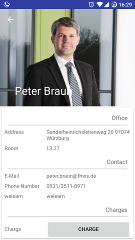
\includegraphics[width=0.4\textwidth]{images/detail.png}
		\caption{Beispiel einer DetailView eines Dozenten nach Material Design Guidelines}
		\label{fig:detail}
	\end{center}
\end{figure}

Die zur Verfügung  stehenden Daten sind die gleichen, welche unter Listing \ref{lst:braun_json} einzusehen sind.

Analog wie bei der CardView stellen Sich auch bei der DetailView, welche Daten alle dargestellt werden sollen. Hier jedoch gibt es zusätzlich zu der horizontalen Gruppierung (Beispiel mit den Vornamen und Nachnamen), auch noch eine vertikale Gruppierung, die im weiteren auch Kategorisierung genannt wird. In der detaillierten Ansicht eines Dozenten gibt es die Möglichkeit die Attribute zu kategorisieren und jeder Kategorie mit einem Namen zu versehen. Für die Gestaltung und Anordnung sowie mögliche Klick-Aktionen müssen die selben Anforderungen wie bei der CardView berücksichtigt werden. 

Jedoch muss die DetailView wissen, welches Attribut den Titel der View darstellt, da dieser in der AppBar erscheinen wird. In diesem Beispiel ist es der Name des Dozenten. Anders als bei der CardView gibt es hier nicht die Möglichkeit zu bestimmen wo das Bild dargestellt werden soll. Ist ein Bild vorhanden, so wird dieses in der Collapsing-Toolbar dargestellt \cite{collapsing}. Andernfalls wird kein Bild angezeigt.

\subsubsection{InputView}

\begin{figure}[H]
	\begin{center}
		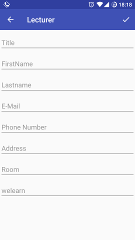
\includegraphics[width=0.4\textwidth]{images/input.png}
		\caption{Beispiel einer View zum Anlegen eines Dozenten}
		\label{fig:input}
	\end{center}
\end{figure}

Für das neu Anlegen eines Dozenten oder auch zum bearbeiten muss entschieden werden, welche Attribute zum Anlegen benötigt werden. Auch hier ist es notwendig die Reihenfolge zu bestimmen. Jedoch kommen in dieser View für jedes Attribut noch die Möglichkeit hinzu ein Hint-Text anzugeben. Dieser Text beschreibt, was in der Android View EditText als Beschreibung für das bestimmte Attribut steht. Weiter sollte es die Möglichkeit geben, jedem Feld eine Nachricht mitzugeben, welche Angezeigt wird, wenn das Feld beispielsweise leer gelassen wird. Oder eine weitere Nachricht, wenn das Eingegebene nicht dem Erwarteten entspricht. Zum Beispiel wurde in das Feld für die E-Mail die Telefonnummer eingegeben. Oder es wurde ein regulärer Ausdruck mitgegeben und das Eingegebene entspricht nicht den Anforderungen, welche durch den regulären Ausdruck definiert wurden.

\subsubsection{Programmablauf und Klick-Aktionen}

Da das Enfield-Model bereits einen endlichen Automaten beschreibt, welcher den Programmablauf widerspiegelt, ist es nicht notwendig, diesen Ablauf noch einmal genauer zu definieren. Da der bereits definierte Ablauf übernommen wird.

Auch die Klick-Aktionen, das Geschehen, welches durch einen Klick auf ein bestimmtes Attribut ausgeführt werden soll, beschränkt sich auf Android Standard Aktionen. Beispielsweise das wechseln zu den Maps, zu einem E-Mail Client, dem Browser oder zum Anrufsmenü. Jede deser Aktion ergibt sich aus den Typen der Attribute, weswegen diese auch nicht weiter definiert werden müssen.

\subsection{Design der View-Meta-Modelle} \label{sec:resourceViews}

In den letzten Abschnitten der Arbeit wurde aufgezählt, was das Meta-Model alles Abdecken muss und das sowohl Android- als auch Polymer-seitig. In diesem Kapitel wird ein Meta-Model vorgestellt, welches die erwähnten Eigenschaften abdeckt.


\begin{figure}[H]
	\begin{center}
		\includegraphics[width=\textwidth]{images/metamodel.png}
		\caption{Aufbau der Views zur Erweiterung des Enfield-Models}
		\label{fig:meta-model}
	\end{center}
\end{figure}

Die Abbildung \ref{fig:meta-model} zeigt den Aufbau der Objekte, mit welchem das Enfield-Model erweitert wird. Die drei Views CardView, DetailView und InputView sind alles Instanzen von AbstraktResourceView. Jede der View, weiß welche Ressource sie darstellen soll. Dies passiert über die Zuordnung mit Hilfe des Ressourcennamens. Die drei Views, lassen sich in zwei Kategorien einteilen: Views, welche Informationen anzeigen und Views welche zur Eingabe von Informationen benötigt werden.
So gehören CardView und DetailView zur anzeigenden Views und die InputView zur zweiten Kategorie. 

\subsubsection{Anzeigende Views}
Diese View-Typen haben die Aufgabe in einer Liste alle Attribute zu halten, welche in der entsprechenden View angezeigt werden sollen. Dabei bestimmt die Reihenfolge, in welcher die Attribute in dieser Liste sind auch die Anordnung in der Oberfläche. Ist das erste Item in der Liste der Name, so wird dieser ganz oben in der View angezeigt.
Bei der DetailView jedoch gibt es nicht eine Liste mit den Attributen, sondern eine Liste mit Kategorien. Diese Kategorien, besitzen 
einen Namen und eine Liste mit den Attributen ihrer Kategorie. Die Darstellungsreihenfolge der Kategorien und deren Attribute ist analog zu der der CardView. Weiter besitzt die DetailView das Attribute \textit{image}, dieses Attribut wird hier aus der Liste der Attribute herausgezogen, da dieses Attribut bestimmt, ob die View eine Collapsing-Toolbar besitzen wird oder nicht. Wiederum haben beide Views das Attribut \textit{titleOfResource} dieses bestimmt welches Attribut unserer Ressource beispielsweise in der Toolbar angezeigt wird.

Auf die Polymer-spezifischen Attribute wird in dieser Arbeit nicht weiter eingegangen.

Mit Hilfe der Listen, Titelattributen und dem Bildattribut kann das Erscheinungsbild einer View schon ziemlich gut beschrieben werden. Jetzt bleibt fehlt noch die Möglichkeit, die Schriftgrößen, Schriftfarben, Klick-Aktionen und so weiter zu definieren.
Außerdem ist es bis jetzt nur möglich einfache Attribute anzuzeigen, eine horizontale Gruppierung ist noch nicht möglich. Um diese Anforderungen zu erfüllen, werden nicht Attribute in den Listen gespeichert sondern Ausprägungen von ResourceViewAttributen. 

Es gibt zwei Ausprägungen: ein SingleResourceViewAttribute und ein GroupedResourceViewAttribute.  Das SingleResourceViewAttribute ist für einfache Attribute, mit diesem ist es beispielsweise möglich den Titel eines Dozenten anzuzeigen. Das GroupedresourceViewAttribute ermöglicht die horizontale Gruppierung. Beide Objekte, bestimmen jedoch nicht die Design-spezifischen Eigenschaften des Attributs. Hierfür besitzen beide Attribut-Typen das Attribut DisplayViewAttribute.

Bei der SingleResourceViewAttribute ist diese Instanz von einem AbstractViewAttribute das einzige Attribut, beim GroupedResourceViewAttribute wiederum gibt es eine Liste von diesen DisplayViewAttributen, welche dann die anzuzeigenden Informationen widerspiegeln. Weitergehend besitzt diese Attribut-Art auch noch ein DisplayViewAttribute, welches die neu entstandene Gruppierung beschreiben soll.

Ein DisplayViewAttribute besitzt nun die Möglichkeit, die Schriftgröße und -farbe zu definieren. Die angegebene Farbe muss eine Farbe in hexadezimaler Darstellung sein, wird keine Farbe mitgegeben, wird die Default-Farbe der Anwendung genommen. In der Regel ist diese Schwarz.  Die Schriftgröße wiederum ist auf 3 Stufen beschränkt. Es gibt die Möglichkeit den Text in klein, normal und groß darzustellen. Per default ist normal eingestellt. Aus der Oberklasse AbstractViewAttribute besitzt das DisplayViewAttribute noch die Attribute \textit{attributeName}, dieses muss exakt so heißen wie in der Definition der Ressource beschrieben.
Mit dem \textit{attributeLabel} kann angegeben werden, wie dieses Attribut in der View angezeigt werden soll. Die Abbildung \ref{fig:detail} zeigt die Verwendung von den Labels, vor beispielsweise der E-Mailadresse des Dozenten steht \textit{E-Mail}, dieser String entspricht dem Label des Attributes. Muss angeben werden von welchem Typ das aktuell beschriebene Attribut ist.
Dies geschickt mit dem Attribut AttributeType. Es gibt folgende mögliche Typen: HOME, MAIL, LOCATION, PICTURE, PHONE\_NUMBER, TEXT, URL, DATE, SUBRESOURCE. Jeder Typ bestimmt die Eigenschaften des Attributes. Über diesen wird bestimmt welches Icon in der Karte vor dem entsprechenden Attribut angezeigt werden. Auch bestimmt er welche Aktion bei Klick ausgeführt werden soll. So wird bei einem Klick auf ein Attribut vom Typ LOCATION versucht die Anwendung Maps zu öffnen und den angezeigten Standort dort anzuzeigen. Ist das Attribute vom Typ SUBRESOURCE so wird für dieses Attribut ein Button angezeigt, dieser ermöglicht es dann zu der entsprechenden Subressource zu wechseln. Diese Klick-Aktionen müssen jedoch mit dem Attribut \textit{clickActionAndroid} erst aktiviert werden.

Manche Typen bringen noch ein paar andere Besonderheiten mit sich. So muss man beispielsweise bei einem URL-Attribut noch eine Beschreibung mitgeben, welche anstelle der Hyperlinks angezeigt werden soll. Bei einem Bild kann man beispielsweise noch bestimmen, ob dieses links oder rechts dargestellt werden soll. 

Das im Anhang befindliche Listing \ref{lst:detailview_impl} zeigt die Definition einer DetailView.

\subsubsection{Eingebende Views}

Bei der InputView gibt es wieder eine Liste, welche dieses mal InputViewAttribute mit der Oberklasse AbstractViewAttribute hält. Diese Liste bestimmt analog zu den anzeigenden Views die darzustellende Reihenfolge der Attribute. 

Neben dem \textit{attributeName} der wieder exakt dem Namen aus der Ressourcendefiniton entsprechen muss, besitzt das InputViewAttribute auch die Möglichkeit zu bestimmen, welcher Typ das aktuelle Attribut besitzt. Jedoch haben die Typen hier eine Andere Bedeutung als bei dem anderen View-Typ. So wird beispielsweise bei dem Type DATE kein EditText angezeigt, sondern der Nutzer hat die Möglichkeit das Datum über das DatePicker-Widget von Android einzugeben. 

Es ist jedoch für den Android-Client nicht möglich Bilder zu Ressourcen hinzuzufügen, oder diese zu Bearbeiten. Wird eine Subressource nicht in einer InputView der Oberressource bearbeitet oder neu angelegt. Dies ist dann in der entsprechenden View der Subressource möglich. Die anderen Typen beschränken das EditText-Widget auf die angegebenen Typen. So wird bei einem Klick auf ein PHONE\_NUMBER-Feld die Tastatur im Zahlenmodus ausgefahren und so weiter.

Einem InputViewAttribute muss zusätzlich ein \textit{hintText} mitgegeben werden, der im EditText des Attributs beschreibt, was in diesem Feld erwartet wird. Mit dem String \textit{missingText} kann dem Attribut mitgegeben werden, welche Nachricht dem Nutzer angezeigt wird, falls er versucht zu speichern ohne das entsprechende Feld auszufüllen. Mit der Kombination von \textit{checkPattern} und \textit{errorText} bekommt der Nutzer des Generators die Validierung des eingegebenen Attributes noch weiter zu verfeinern und auch dem Nutzer der Applikation ein Feedback zu geben, falls eine falsche Eingabe getätigt wurde.

Die Definition einer InputView wird im Anhang unter Listing \ref{lst:inputview_impl} dargestellt.

\subsection{Analyse und Design von allgemeinen Daten für eine Anwendung}

Dieses Kapitel behandelt die Informationen, welche eine Applikation neben den View-Beschreibungen zusätzlich benötigt, aber diese vom Kontext her nicht in einer der Views beschrieben werden können.

Ein Beispiel für eine solche Information wäre der \acf{url} für den Einstieg. Die Applikation benötigt diesen um zu wissen, unter welcher Adresse sich die anzuzeigenden Informationen zu finden sind. Ein weiteres Beispiel sind die Grundfarben der Applikation. Das Material Design gibt drei benötigte Grundfarben vor: \textit{colorPrimary}, \textit{colorprimaryDark} und \textit{colorAccent} diese Grundfarben wird um die Farbe für den Toolbar-Text erweitert.

Mit dem Wissen, konnte eine Erweiterung des Enfield-Models designed werden, welches in Abbildung \ref{fig:appspecifics} dargestellt ist.

\begin{figure}[H]
	\begin{center}
		\includegraphics[width=0.86\textwidth]{images/appspecifics.png}
		\caption{Aufbau des AppSpecifics Objekt  zur Erweiterung des Enfield-Models.}
		\label{fig:appspecifics}
	\end{center}
\end{figure}

 Über die Map \textit{additionalInformation} können zusätzlich weitere allgemeine Informationen an den Generator, zur Erzeugung der Anwendung, weitergegeben werden .

\section{Software-Generator}

Nachdem das Meta-Model nun klar ist, geht dieses Kapitel der Ausarbeitung auf die Funktionsweise des Generators ein. 
Es wird dargelegt wie der Generator aufgebaut ist und teilweise darauf eingegangen wieso dieser Weg der Generation gewählt wurde. Des weiteren wird das Java \acf{api} JavaPoet kurz vorgestellt \cite{poet}.

\subsection{JavaPoet}
JavaPoet ist ein Java \ac{api}, welches ermöglicht Java-Klassen zu generieren \cite{poet}. Hierfür wird die zu generierende Klasse programmiert. Mit Hilfe von nur ein paar Schlüsselwörtern ist es recht einfach möglich Klassen, Interfaces oder Methoden zu generieren. 

Da der größte Teil des Generators Java-Klassen erzeugen muss, ist dieses \ac{api} bestens für diesen Zweck geeignet. Sie erspart die aufwändige String-Manipulation. Durch die Nutzung wird auch bei der Ausführung des Programmes sichergestellt, das gültige Konventionen und Regeln eingehalten werden. So ist der grundsätzliche korrekte Aufbau einer Java-Klasse bereits sichergestellt.

Listing \ref{lst:poet} zeigt ein einfaches Beispiel zur Generierung einer Hello-World-Klasse und Listing \ref{lst:poet_result} zeigt das Ergebnis nach der Ausführung des Beispieles.

\begin{lstlisting}[label=lst:poet,
language=java,
firstnumber=1,
caption=Beispiel für die Generation einer Hallo-World-Klasse \cite{poet}.]				   
MethodSpec main = MethodSpec.methodBuilder("main")
	.addModifiers(Modifier.PUBLIC, Modifier.STATIC)
	.returns(void.class)
	.addParameter(String[].class, "args")
	.addStatement("$T.out.println($S)", System.class, "Hello, JavaPoet!")
	.build();

TypeSpec helloWorld = TypeSpec.classBuilder("HelloWorld")
	.addModifiers(Modifier.PUBLIC, Modifier.FINAL)
	.addMethod(main)
	.build();

JavaFile javaFile = JavaFile.builder("com.example.helloworld", helloWorld)
	.build();
\end{lstlisting}

\begin{lstlisting}[label=lst:poet_result,
language=java,
firstnumber=1,
caption=Ergebnis der Generation von Listing \ref{lst:poet} \cite{poet}.]				   
package com.example.helloworld;

public final class HelloWorld {
	public static void main(String[] args) {
		System.out.println("Hello, JavaPoet!");
	}
}
\end{lstlisting}

\subsection{Generierung anderer Daten-Typen}

Neben Java-Klassen besitzt der Sourcecode einer Android Applikation auch XML-Dateien und Gradle-Dateien. Für diese Typen muss eine andere Möglichkeit der Generierung gewählt werden. Hierfür liefert \acf{gemara} mit der Klasse GeneratedFile eine Möglichkeit. Diese Klasse liefert die die beiden Methoden \textit{append(String contet)} und \textit{appendln(String content)}. Welche es ermöglichen jedes beliebige textbasiertes File-Format zu generieren. Ein GeneratedFile Objekt erzeugt eine Datei, welcher mit den beiden erwähnten Methoden Strings hinzugefügt werden können, dies ermöglicht es jede beliebige Textstruktur zu erzeugen. Jedoch liefert diese Klasse keinerlei Validierung, die Datei wird generiert egal ob die Struktur gültig ist oder nicht.

So würde Listing \ref{lst:append} eine Datei \textit{test.xml} im Verzeichnis \textit{generated} erzeugen. Diese erzeuge Datei wird in Listing \ref{lst:append_result} dargestellt.

\begin{lstlisting}[label=lst:append,
language=java,
firstnumber=1,
caption=Beispiel eine GeneratedFile-Instanz zur Erzeugung einer XML-Datei.]				   
public class FileGenerator extends GeneratedFile {

	@Override
	public void generate() {
		appendln("<?xml version=\"1.0\" encoding=\"utf-8\"?>");
		appendln("<menu xmlns:android=\"http://schemas.android.com/apk/res/android\" xmlns:app=\"http://schemas.android.com/apk/res-auto\">");
		appendln("<item android:id=\"@+id/saveItem\"");
		appendln("android:title=\"@string/save\"");
		appendln("app:showAsAction=\"always\"\\>");
		appendln("<\\menu>");
	}

	@Override
	protected String getFileName() {
		return "test.xml";
	}

	@Override
	protected String getDirectoryName() {
		return "/generated";
	}
}
\end{lstlisting}

\begin{lstlisting}[label=lst:append_result,
language=xml,
firstnumber=1,
caption=Erzeugte XML-Datei durch den Quellcode von Listing \ref{lst:append}.]				   
<?xml version="1.0" encoding="utf-8"?>
	<menu xmlns:android="http://schemas.android.com/apk/res/android"
		xmlns:app="http://schemas.android.com/apk/res-auto">
		<item android:id="@+id/saveItem"
			android:title="@string/save"
			android:icon="@drawable/ic_done"
			app:showAsAction="always"/>
	</menu>
\end{lstlisting}

\subsection{Aufbau der zu generierenden Applikation}

Um den Generator möglichst zu vereinfachen, ist es hilfreich, eine Referenzimplementierung der gewünschten Applikation mit all ihren Funktionen und Anforderungen zu entwickeln. Bei einer anschließenden Quellcode-Analyse sollte darauf geachtet werden, die einzelnen Klassen soweit zu abstrahieren, das eine Einteilung in generischen und spezifischen Quellcode erfolgen kann. Der generische Quellcode ist einfacher zu generieren, da dieser statisch ist und sich für alle folgenden Implementierungen nicht verändert. Es können auch Überlegungen angestrebt werden, diese generischen Klassen einfach im Generator abzulegen und bei Bedarf zu kopieren. Diese Methode wurde verworfen, da sich andernfalls jedes mal die kopierten Klassen via String-Manipulation bearbeitet werden müssten. Die minimale Änderung welche jedes mal getroffen werden müsste, wäre das Anpassen der Package Anweisung am Anfang der Java-Klassen und die Anpassung der Import-Anweisungen. Eine weitere Überlegung wäre es, diese Klassen in eine Android Bibliothek auszulagern, und diese dann in jede Anwendung zu importieren. Auch von dieser Möglichkeit wurde in der ersten Version abgesehen, da die Applikation bereits aus zwei Komponenten besteht. Der Applikation an sich und einer Bibliothek, welche die Android-Komponenten für die Anwendung enthält. Um die Komplexität zu reduzieren werden die benötigten generischen Klassen als Teil der eingebunden Bibliothek jedes mal aufs neue generiert.

Die Referenzimplementierung für diese Arbeit beinhaltet folgende Features:
\begin{center}
	\begin{tabular}{p{0.4\textwidth}|p{0.4\textwidth}}
		\textbf{Ressource: Dozent} & \textbf{Ressource: Amt} \\ \hline
		\begin{itemize}
			\item Anzeige einer Liste mit Dozenten
			\item Anlegen neuer Dozenten
			\item Anzeigen eines Dozenten in Detail
			\item Bearbeiten eines Dozenten
			\item Löschen eines Dozenten
		\end{itemize}
		&
		\begin{itemize}
			\item Anzeigen einer Liste von Ämtern eines Dozenten
			\item Anlegen neuer Ämter für einen Dozent
			\item Anzeigen eines Amtes eines Dozenten
			\item Bearbeiten eines Amtes eines Dozenten
			\item Löschen eines Amtes eines Dozenten
		\end{itemize}
		\\
	\end{tabular}
\end{center}

Der Aufbau der Referenzimplementierung wird in Abbildung \ref{fig:lecturer} dargestellt. Das Schaubild verdeutlicht das Verhältnis von generischen (weiße Kästen) und spezifischen (rote Kästen) Klassen. Die Anzahl der gleichbleibenden Klassen ist mit etwa 60 Prozent bereits höher als der Anteil an spezifischen Klassen. Je höher der Anteil dieser unveränderlichen Klassen, desto geringer wird die Komplexität des Generators. Da der Aufwand eine spezifische Klasse zu erzeugen mehr Logik benötigt, als eine Klasse, welche immer gleich bleibt.

Daneben zeigt die Abbildung \ref{fig:lecturer} aus dem Anhang, auch noch die Aufteilung der Klassen in Klassen der Applikation (gestrichelte Kästen) und Klassen der Bibliothek (solide Kästen). Die Applikation an sich besteht nur aus ein paar wenigen Fragmenten und Aktivities, welche alle projektspezifisch sind. Der komplette generische Quellcode befindet sich in der Bibliothek. Des weiteren befinden sich dort auch die spezifischen Komponenten, beispielsweise der \textit{LecturerInputView}. Diese Komponente, kann in den Fragmenten zur Bearbeitung oder Neuanlage eines Dozenten dann mit wenigen Zeilen Programmcode verwendet werden.

Diese Art der Aufteilung ermöglicht es das ein Applikation Entwickler sich die Komponente, für das Anzeigen, Bearbeiten, Löschen und der Neuanlage generieren lassen kann. Diese Komponenten jedoch beliebig in seiner eigenen Applikation verwenden kann.

\subsection{Aufbau des Generators}

\begin{figure}[H]
	\begin{center}
		\includegraphics[width=\textwidth]{images/Welling.png}
		\caption{Aufbau des Android-Generators Welling}
		\label{fig:welling}
	\end{center}
\end{figure}


Die Klasse ApplicationGenerator, ist der Einstiegspunkt des Projekts. Sie erwartet im Konstruktor ein Enfield-Model Objekt. Wie der Abbildung \ref{fig:welling} entnommen werden kann, so lässt sich das Projekt in drei Teilbereiche gliedern. Der erste Bereich erzeugt ein AppDescription Objekt (Abbildung \ref{fig:appDescription}) der zweite Bereich befasst sich mit allgemeinen Vorbereitungen, die getroffen werden müssen. Der Letzte iteriert über die States, und generiert nach bedarf die benötigten Klassen.

Die ApplicationGenerator Klasse verfügt über eine öffentliche Methode \textit{generate}. Beim Aufrufen dieser Methode, werden die einzelnen Generatoren, für den allgemeinen Bereich angestoßen. Weiterhin wird das iterieren über die States des Enfield-Model begonnen. Zum Schluss wird noch das AppDescription Objekt ausgewertet, und die darin enthaltenen Informationen in Dateien geschrieben und an die entsprechende Stelle im Projekt gespeichert.

\subsubsection{Erstellung der AppDescription}

\begin{figure}[H]
	\begin{center}
		\includegraphics[width=\textwidth]{images/AppDescription.png}
		\caption{Aufbau des AppDescription Objekts.}
		\label{fig:appDescription}
	\end{center}
\end{figure}

In der AppDescription werden alle Daten durch den Generator gereicht, welche an vielen Stellen benötigt werden. 
An vielen Stellen wird beispielsweise dir Name der Anwendung oder der Bibliothek benötigt. In jeder Java-Klasse wird der Paket Name benötigt, da dieser in der Bibliothek und in der normalen Applikation verschieden sind müssen diese für beide mitgeführt werden. Auch muss der Generator wissen, unter welchen Verzeichnissen die aktuelle Datei egal ob Java Klasse oder XML-Datei gespeichert werden soll. 
Diese Dateien können einfach aus dem Enfield-Model abgelesen werden. Auch die Ressourcen und die jeweiligen Subressourcen können direkt aus dem Meta-Model entnommen werden.  Dies ist der Teil des initialisieren der AppDescription. Alle bereits jetzt verfügbaren Informationen werden der AppDescription zugewiesen. 

Neben diesen Daten, die an mehreren Stellen bei der Generierung benötigt werden, gibt es Dateien in einer Android-Applikation, die sich mit dem Generieren aufbauen. Ein Beispiel für eine solche Datei ist die \textit{strings.xml}. 
Es wird in dem generierten Projekt zwei davon geben. Eine im Bereich der Applikation selbst und eine weitere im Bereich der Bibliothek. Diese Dateien enthalten neben dem Applikationsnamen beziehungsweise des Bibliotheksnamen auch viele Strings, die erst beispielsweise in einem Fragment auftauchen. Jedoch müssen die benötigten Datensätze in der \textit{strings.xml} eingetragen werden. Anstelle dies jedes mal wenn im Ablauf des Generierens ein String auftaucht, eine bereits generierte Datei zu erweitern, wird der Datensatz in der AppDescription unter dem AppString \textit{appString} beziehungsweise dem AppString \textit{libString} hinterlegt.

Auch das AndroidManifest wächst mit der Anwendung. So muss jede benutzte Aktivity dort eingetragen sein. Andernfalls kann diese nicht genutzt werden. Am Anfang des Generierens ist die genaue Anzahl und die genauen Namen der Aktivities unbekannt, weswegen der Generator diese beim Erzeugen zur AppDescription hinzufügen muss. 

Das Attribut \textit{appDeclareStyleable} enthält alle Custom Attribute, welche wie, im Kapitel \ref{sec:custom_view}, in die \textit{attr.xml} eingetragen werden müssen.

Da die Anwendung, welche generiert wird auch den \acf{rest} Ansätzen entsprechen soll, muss diese wissen welche Relationstpyen zu welchen Endpunkten gehören. Anfangs sind diese jedoch auch unbekannt und werden erst im weiteren Verlauf beim iterieren über die States bekannt und zur AppDescription hinzugefügt.

So wächst die AppDescription über den gesamten Prozess des Generierens. Ganz am Ende, werden die gesammelten Daten in die entsprechenden Dateien an den jeweiligen Orten gespeichert. Das Verwenden und weiterreichen eines AppDescription Objekts reduziert die Komplexität des Generators. Dieser muss nicht bei jeder Ergänzung einer der beschriebenen Dateien diese Aufrufen, den neuen Datensatz aufwändig hinzufügen und die Datei wieder abspeichern. Sondern der Generator muss nun die Datei nur einmal schreiben, da er jetzt alle von der Android Anwendung benötigten Informationen besitzt.

\subsubsection{Vorbereitung und Generierung allgemeiner Dateien}

Der Bereich zur Vorbereitung und Generierung der allgemeinen Dateien gliedert sich ebenfalls in 3 Bereiche. Der erste Bereich kümmert sich um alle Dateien die von Gradle benötigt werden. 

Er kopiert Daten wie die \textit{gradlew.bat}, \textit{gradlew}, \textit{build.gradle} und den Gradle Wrapper. 
Neben dem Kopieren, werden sowohl für die Applikation, Bibliothek als auch für das Gesamtprojekt die spezifischen Dateien generiert. So wird beispielsweise auf der Projektebene eine \textit{settings.gradle} erzeugt oder in der Applikation sowie in der Bibliothek jeweils eine \textit{build.gradle}.

In der Sektion der Vorbereitung für die Applikation an sich, werden Dateien erzeugt, die jede Applikation benötigt unabhängig von ihrem Aufbau oder den Features. Es wird beispielsweise die MainActivity erzeugt, oder die XML-Dateien, welche für die Transitionsanimationen verantwortlich sind. Auch die \textit{styles.xml} wird erzeugt. Am Schluss werden noch die \textit{mipmap}-Ordner kopiert und an die richtige Stelle verschoben.

Der Bereich, welcher die Bibliothek initialisiert, ist der Größte. Er generiert alle generell benötigten Klassen. Darunter fallen die Klassen für die Netzwerkkommunikation, Die Klasse für das Link-Objekt sowie das Interface \textit{Resource}. Es werden des  werden auch die größten Teile der in der Abbildung \ref{fig:lecturer} abgebildeten generischen Klassen erzeugt. Auch werden die grundsätzlichen CustomViews bereits erzeugt. Dazu gehören auch noch die benötigten XML-Dateien. So kann für die Bibliothek beispielsweise das Manifest bereits erzeugt werde, da hier keine Activities registriert werden müssen. Nach dem Ausführen des \textit{PrepareLibGenerators} steht, das Grundgerüst der Bibliothek. Diese enthält nun alle bereits vorab erzeugbaren und benötigten Dateien, welche unabhängig von der gewünschten Funktion der Applikation benötigt werden. 

Dieser gesamte Teilbereich des Projekts befasst sich damit ein Grundgerüst für die komplette Android Applikation zu erzeugen und vorab bereits alle benötigten Dateien bereit zu stellen. Die generierten Klassen haben jedoch noch keinerlei Programmlogik, die den spezifischen Ablauf der zu generierenden Anwendung steuert.

\subsubsection{Iterieren über die States}

Der Teilbereich, der sich mit dem iterieren über die einzelnen States beschäftigt ist der komplexeste Bereich des Generators. Er ist dafür verantwortlich, das zu jedem State die alle benötigten Klassen und Dateien generiert werden. 

Um diese Anforderung zu erfüllen, nutzt er den Visitor \textit{IStateVisitor}, welcher durch das Enfield-Model zur Verfügung gestellt wird. Außerdem wird auch der Visitor \textit{VisitStatesOnlyOnce} benutzt. Dieser zweite Visitor stellt sicher, das jeder State nur einmalig Besucht wird. Würde der Generator einfach nur über die Transitionen der States gehen, könnte es passieren, das er in eine Endlosschleife gerät.

Gelangt der Generator zu einem State, wird mit dem \textit{ISateVisitor} identifiziert, von welchem Typ dieser ist. Ist es ein State, welcher einen GET-Request auf eine einzelne Ressource oder auf eine Collection beschreibt, oder beschreibt er einen POST-, PUT- oder DELETE-Request.  Nach dieser Identifikation, wird bei jedem State, außer dem DELETE-State, eine Klasse für die in diesem State betroffene Ressource erzeugt. Hierfür wird der \textit{ResourceGenerator} benutzt. Auch wenn dabei die Ressource mehrfach angelegt werden würde. Der Generator überschreibt eine bereits angelegte Ressource einfach. Diese Redundanz garantiert das auf jeden Fall eine Ressource zum betreffenden State existiert. 

Neben diesen Ressource-Klassen, wird auch ein StateHolder-Objekt erstellt. Die Abbildung \ref{fig:stateHolder} repräsentiert dieses. 

\begin{figure}[H]
	\begin{center}
		\includegraphics[width=0.3\textwidth]{images/StateHolder.png}
		\caption{Aufbau des StateHolder Objekts.}
		\label{fig:stateHolder}
	\end{center}
\end{figure}

Dieses Objekt wird für jeden einzelnen State angelegt, es enthält alle States, welche über die Transitionen erreicht werden können.
So weiß der Generator genau, ob beispielsweise ein Button angezeigt werden muss, der eine Neuanlage einer Ressource ermöglicht. Diese Informationen stecken zwar auch im Enfield-Model, jedoch müsste jedes mal wenn überprüft werden soll welche Folgestates ein State besitzt, über alle States iteriert werden. Das StateHolder-Objekt beschreibt sozusagen eine Landkarte für jeden einzelnen State.

Der State, welcher für das Löschen einer Ressource verantwortlich ist, ist der einfachste zum generieren. Hierfür muss nur ein DialogFragment erzeugt werden, der für das Löschen verwendet wird. 

Für die anderen States, werden mehr Klassen und Dateien benötigt. Außerdem werden die ResourceViews (Kapitel \ref{sec:resourceViews}) benötigt, die jedem State angehängt sind. Zur Identifizierung der einzelnen ResourceViews wird wiederum mit dem Visitor-Pattern gearbeitet. Die Klasse der ResourceView stellt den Visitor \enquote{ResoruceViewVisitor} zur Verfügung. 
Nachdem bekannt ist welche der drei ResourceView-Typen im entsprechenden State verwendet wurde, kann einer der Komponentengeneratoren: InputViewGenerator, CardViewGenerator oder DetailViewGenerator alle notwendigen Dateien generieren.

\begin{figure}[H]
	\begin{center}
		\includegraphics[width=\textwidth]{images/Lecturer-Swimlines.png}
		\caption{Aufbau der Dozenten Applikation mit Einteilung in spezifische States.}
		\label{fig:swimlines}
	\end{center}
\end{figure}

In Abbildung \ref{fig:swimlines} ist die Applikation für Dozenten noch einmal abgebildet. Zur Vereinfachung wurde bei diesem Diagramm jedoch die Ressource Ämter mit ihren zugehörigen Klassen weggelassen.

Der Bereich \enquote{Update} und der Bereich \enquote{Create} werden hierbei vom InputViewGenerator, der Bereich \enquote{Read Collection} von CardViewGenerator und der Bereich \enquote{Read Single} vom DetailViewGenerator erzeugt.

Jeder der einzelnen Generatoren ist ein Zusammenschluss von vielen Teilgeneratoren. Es werden dabei in einem der Generatoren nicht nur die Java-Klassen für die Applikation oder die Bibliothek, sondern auch alle benötigten XML-Dateien erzeugt.

So ist beispielsweise der DetailViewGenerator dafür verantwortlich, dass auf der Seite der Applikation, die \enquote{LecturerDetailActivity} inklusive ihrer XML-Datei erzeugt wird. Er muss weitergehend auch diese Aktivity in die AppDescription im Bereich des Manifestes hinterlegen. Im Bereich der Bibliothek muss dafür gesorgt werden, dass die generischen Klassen \enquote{ResourceDetailActivity}, \enquote{ResourceDetailView} sowie die spezifischen Klassen: \enquote{LectuererDetailView}, \enquote{LectuererDetailAdapter}, \enquote{LectuererDetailViewHolder}, \enquote{LectuererDetailCardView} erzeugt werden. Zu all diesen Klassen müssen mögliche Strings oder CustomViews in die AppDescription aufgenommen werden. Wiederum müssen auch die entsprechenden XML-Dateien erzeugt werden. 

Jeder Generator besitzt mehrere Möglichkeiten, welche Klassen generiert werden müssen. So entscheidet beispielsweise ob die Ressource ein Bild besitzt oder nicht über den Verhalt, ob eine Activity mit einer CollapsingToolbar verwendet wird oder ob ein einfaches Fragment zur Detailanzeige ausreichend ist.

Selbst die Generatoren auf der untersten Ebene, welche die einzelne Klassen erzeugen, wissen mit Hilfe von dem mitgegebenen StateHolder, ob beispielsweise Menüeinträge für das Löschen oder das Bearbeiten von Ressourcen benötigt werden. Diese Generatoren richten sich auch nach den übergebenen RessourceViews. Auf dieser Ebene haben die vom Benutzer des Generators mitgegebenen Informationen zum Aussehen, Einfluss. Hier werden die benötigten Attribute der Ressource hinzugefügt, und deren Aussehen in den entsprechenden XML-Dateien beschrieben.


\section{Bauen und ausführen der generierten Android Applikation}

Wurden alle benötigten Dateien der Applikation erzeugt, gibt es zwei Möglichkeiten, die Applikation zu bauen und anschließend auf einem Android-Endgerät zu installieren.

Variante 1: Importieren der generierten Dateien in eine \acf{ide} beispielsweise in Android Studio. Dort wie bereits bekannt, die Anwendung bauen und auf einem sich im Entwicklermodus befindlichen Android-Endgerät installieren.

Variante 2: Die Applikation mit Hilfe des Makefile bauen und installieren. Hierfür muss ebenfalls ein Android-Endgerät im Entwicklermodus an dem entsprechenden Computer angeschlossen sein.

\newpage

\begin{lstlisting}[label=lst:make,
language=xml,
firstnumber=1,
caption=Makefile für das Bauen und Installieren der erzeugten Applikation.]				   
APK = gemara/android/src-gen/generated/app/build/outputs/apk/app-debug.apk

all: debug install

debug:
cd gemara/android/src-gen/generated && chmod 777 gradlew && ./gradlew clean assembleDebug

install:
adb $(TARGET) install -rk $(APK)
\end{lstlisting}

Listing \ref{lst:make} zeigt das Makefile, dieses bietet die Möglichkeit entweder mit dem Befehl \textit{make} eine Debug-Version der Anwendung zu bauen und zu Installieren, oder mit dem Befehl \textit{make debug} ausschließlich die Applikation zu bauen beziehungsweise mit dem Befehl \textit{make install} die bereits gebaute Applikation zu installieren.
